\chapter{What Kind of War Is This?}
Small wars, like the poor of the bible, are always with us. Since the end of World War II each year has seen an average of 40 small wars occuring around the globe. People have been killing each other with all sorts of technology from primitive weapons such as spears and swords to the most recent innovations such as Soviet Hind helicopters firing guided missiles. Nuclear weapons have not yet been employed, but there is no certainty that they will not be.

Although many years have elapsed since the first use of nuclear weapons in war, there has never been a nuclear war as the term is popularly understood. Of course in one sense we are already engaged in nuclear war, in that the Technological War has an important nuclear dimension; but nuclear weapons have not been used in anger since before the capitulation of the Japanese.

This has not meant the end of conflict. The United States was heavily engaged in Vietnam, so much so that the level of effort was greater than that put forth in all of our wars with the exception of World War II and the Civil War. The Korean War, although limited, was no small affair; in various other places, such as the Bay of Pigs, U.S. prestige has been heavily involved in the outcome of military operations, not all of which have been successful.

One of the most inhuman wars of the decade of the 1980s has been the Soviet attempt at conquest in Afghanistan. Long delayed in the timetable of Soviet expansion to its coveted warm water port, Afghanistan has yet to fall under the Soviet war machine on its way through Pakistan to the Indian ocean. The struggle between nationalist guerrillas using mostly primitive weapons and the world's mightiest military force employing highly advanced technology was a proving ground for Soviet doctrine, operations, leadership and technology. As they face the next step the Soviets have to anticipate a strategic issue -- would the invasion of Pakistan result in Pakistan using nuclear weapons to halt the onslaught?

As usual, the Soviets have employed a propaganda campaign to "arouse the world against proliferation of nuclear weapons". The assertion that Pakistan needed nuclear bombs as a counter to its powerful neighbor, India, was discounted. Under no circumstances should Pakistan have nuclear weapons to deter the Soviets in the 1990s from marching toward this decades long desired prize.

The world struggle may ultimately be decided in a major nuclear conflict between the United States and the U.S.S.R. Obviously any decision in such a confrontation would determine the fate of the world; but until that final engagement takes place, if it ever does, there will be numerous dispersed brush-fire, limited, police-action, or small wars, and these can be of enormous strategic significance. The outcomes of small wars can contribute to success in centralized war, facilitate or lead to nuclear aggression, or render nuclear battle unnecessary. They are key events in the Protracted Conflict.

\section{Classification of Conflicts}
In this chapter we define and describe Small Wars, relate them to other wars in what is called the spectrum of warfare, examine some of the major issues, and then deal with options for applying technologies to this aspect of the Technological War. We begin with a definition and description.

\section{What Are Small Wars?}
Small wars are a special form of organized violence to seize and maintain political power. Small wars have been part of human affairs for many thousands of years, but in the 20th century the art, science, strategy, tactics and operations of small wars were highly developed and employed by political ideologues.

The conspiratorial revolutionaries, such as Blanqui, in the late 18th and early 19th centuries, developed the tactics, which are incorporated into small wars. Lenin and the Bolsheviks, building on the conspiratorial revolutionaries, introduced a "scientific" approach and with it a strategy for seizing power. Trotsky's operational plan for the capture of St. Petersburg in 1917 became the model for today's operational planning.

Since the 1920's, the Lenin School in Moscow has been teaching conspiratorial revolution and its many tactics and techniques; strategy for seizing power; tactics, such as propaganda and disinformation; and operational use of violence, such as kidnaping, assassination, demonstrations and terrorism. An innovation in the past two decades has been the use of drug traffic as the source of funds for revolutionaries.

The Lenin School in Moscow is no longer the only school for small wars. North Korea, Cuba, East Germany and Czechoslovakia now have centers for training individuals in strategy, tactics, and operations.

In the 19th century, the century of revolution, there were many opportunities to use violence for attempted seizures of political power: In 1848 in France and Germany; and the Paris Commune of 1870. In the 20th century, we have seen the Russian Revolution of 1905, Lenin, Hitler, Mussolini, Castro and Ortega.

The starting point for the "scientific" study of this form of organized violence was the extensive literature of sociologists such as Weber and Mosca, political economists Pareto, and Sorel.

The strategy of such small wars is based on a theory of the power structure of society and government. The key element is the elite which controls the instruments of power, principally the coercive armed forces, the military services, the constabulary and the police. But it includes also communication, transportation and propaganda.

Thus, the struggle is between decision centers, i.e., the elite on the one hand and the group using violence to seize power on the other.

The issue for a strategy of technology is whether that technology should be applied to specific parts of the spectrum of conflict, or should it provide applications flexible enough for all parts of it. A second issue is whether the technology should be acquired to be the counterpart of that of the enemy at a specific level. In other words, can high technology be applied to low intensity wars, and conversely, can low technology be employed at high levels of conflict.

This is obviously an artificial approach because technology, like war, really cannot be defined as a spectrum.

Two cases, Afghanistan and Pakistan, point out the dimension of the strategic problems of small wars and of the strategy of technology involved. The types of conflicts described as small wars encompass terrorism; assassination; marriages of criminal elements, such as dope smugglers, and subversives; large scale guerrilla actions; insurgences; civil wars; and highly intensive conflicts in which advanced technologies from space reconnaissance (used by the Soviets), were applied to electronic warfare used by Israel and Egypt. In the last war between them the overhanging question was, just as it will be when the Soviets invade Pakistan, will nuclear weapons be used?

The technological problems of the American strategist of technology in dealing with small wars are different from those in other countries. The Israelis for example have a clearly defined defensive mission and they are constantly upgrading the applications of advanced technology to their offensive power. The Soviets employ a wide range of conflicts as part of their global expansion and they equip surrogates with many types of technology depending on the location, geography, and forces engaged. Even when expanding into the American domain they have employed surrogates, such as Castro and Ortega, and have equipped them with the technology appropriate for putting them in power and keeping them there. At the same time they have secured bases near the US heartland from which they can operate their forces equipped with their most advanced technology.

As the defensive power the US has developed military forces, alliances, and bases from which to operate against a constantly expanding range of conflicts. On two occasions when operating at the highest level of conflict with conventional weapons, Korea and Viet Nam, the US approached the domain of a major power, the People's Republic of China. The Chinese invasion of Korea raised the strategic issue of whether or not the US would use nuclear weapons. In that situation, Secretary of State John Foster Dulles invoked the policy of "massive retaliation" as a potential US response. In the Viet Nam case, Senator Barry Goldwater was defeated in his bid for the Presidency in 1964 partly because of fear that he would use nuclear weapons. Thus, the array of demands on the American strategist of technology covers technology in all its forms from the highest to the lowest.

The overriding demands of deterring nuclear war have been the engine of the US strategy of technology since the end of World War II when the USSR chose the US as its enemy. Failures to achieve US objectives in large-scale continental war in Korea and Viet Nam have led to high priority for technology for conventional war in Europe. Deterrence with conventional weapons has gone hand-in-hand with nuclear deterrence.

Success in the dynamic struggle to deter large-scale war has not prevented the continual conflicts which threaten the interests of the US and the security of its allies. One consequence was Congressional intervention in 1986 to mandate that the Department of Defense organize and operate "Special Operations Forces" to cope with terrorism, hostage-taking, subversion, guerrilla action, and insurgencies. The problems are global in extent, from Cuba, Nicaragua, El Salvador, Honduras in our own hemisphere; to Angola, Ethiopia in Africa, to Lebanon and Israel in the Middle East, to Afghanistan and Thailand in Asia; and to the Philippines in the Pacific. Threats to our interests and to our allies can best be countered, Congress decreed, if we organize properly.

This is an old argument. In the 1950s the "spectrum of conflict" had theoretical vogue partially because of doctrinal issues such as levels of conflict; escalation of conflict; nuclear thresholds; nuclear firebreaks. The implications for strategy of technology were explored in Project Forecast I in the 1960s. Issues such as "are there technologies which apply to the various levels of conflict" were addressed. Or, if the conflict were at a low level, could it be terminated by employing weapons designed for a higher level of conflict. In other words, would escalating the conflict bring it to an end?

For example, should the long range bomber be employed in a low-level conflict, and if so, when? Conversely, should the risks be run that the "barefoots" equipped with advanced air defense missiles could kill a multi-million dollar aircraft designed for nuclear weapons delivery. Similarly, should counter-insurgency forces be equipped with aircraft designed especially for operating from austere bases in remote areas against small units?

The answer then and for years later was that special forces should not be organized for low level conflicts, and the strategy of technology should not include technologies uniquely for such conflicts.

\begin{mdframed}[backgroundcolor=black!10]
This constraint does not mean that high tech equipment in the inventory should not be employed in small wars. In the Falklands War of 1982 bothe the British and the Argentines employed available weapons such as the "Exocet" missile and Harrier aircraft which had been developed for other wars.
\end{mdframed}

The rationale was two-fold: 1) Forces and tecchnology for higher level conflicts could be employed, and 2) the budget and the priorities required concentration of resources on the two highest requirements -- deterrence of nuclear war, and deterrence of large-scale conventional war in Europe.

The strategy of small wars, like any other strategy, results from the struggle between decision centers. Within the "elite," the group in power, there are at times several groups, coalitions who are trying to displace those who are in control. Thus, within the elite, there is "elite a," "elite b,", "elite c," etc.

Those who are attempting to seize power and who are not part of the elite form a group whose unity of purpose, discipline and control varies from country to country, and time to time. However, what is distinctive is the agreement within the group that the old order, the elite with its several factions, must go.

The observers, victims, targets, and sometimes participants in the struggle are the general population. Their voice, influence and participation in the control of affairs of political, economic and social nature is limited. By and large, the population is neutral in the violent phases of the struggle.

The revolutionaries have many techniques available for "splitting" the elite, and we have been watching them "split" the Congress over U.S. policy in Nicaragua. An indirect approach to the elite is through the population in general. While the group trying to seize power carries on "operations" against the elite and its several factions, and against the general population, its principal target is the instruments of power of the elite, that is, the armed forces, the militia, and the police forces. Most of the members are drawn from the general population, but their loyalty is principally to the ruling "elite." The tactics employed against the instruments of power range from obtaining defection, to assassination, to guerrilla attacks, to large scale military operations. In any seizure of power the role of the military, para-military and police forces is crucial to success or failure.

Finally, the theory and practice of small wars incorporates the intervention of external powers and influence. The most extreme case is that of defeat in war and the imposition of a new controlling elite by the victor. Intervention can also take the form of money, arms, technology, training, and outright, obvious support of the group trying to seize power, such as providing satellite data to them. In the past, such external intervention came from other governments; now it comes also from those who control the international drug traffic.

As we now know the Soviets have come a long way in developing, analyzing, and applying doctrine, strategy, tactics, and operations. Their approach is embodied in Five Laws of War which apply to small wars as well as other forms of war, such as technological war. Their origin lies in the formulation of Lenin of the conditions for seizing power. In today's version, the Five Laws cover Political, Economic, Morale, Technology and Military elements.

The assessment of the laws of war is called the Correlation of Forces. The political element dominates, although until about ten years ago, the military element was primary. There are correlations of political stability, economic power, strength of morale, lead in technology, and related military power. Obviously the status varies from time to time, and the assessment is a dynamic process. But the key point is to exercise control over the dynamic process so as to achieve power. That means planning and organizing.

Assessing the Correlation of Forces is as complex as it is dynamic. The Soviets are not mesmerized by quantitative analysis of status of military forces. True, they employ many models of different levels of conflict, and different sizes of forces. Often, those models are conservative in orientation because the Soviets abhor "adventurism." But quantitative analysis is only a step and often the last step in the process of helping the decision maker. He is a political figure, even the military commander, for he executes policy of the ruling group. He may participate in the decision process itself, but this was not the case under Stalin and even today the military have no vote in the Soviet Defense Council. (The Chief of the General Staff is the Secretary of the Council.)

\section{Political Correlation of the Forces}
The assessment here focuses on the elite in power and its factions. Goals and objectives, strategy, plans (if they exist), and outside political support of the elite are elements of the assessment. The purpose, however, is to understand strengths and weaknesses so as to employ the most effective tactics.

For example, within the elite, a faction may be headed by a dissatisfied close relative of the head of state who may be induced to defect overtly or covertly. In some instances, the church of the predominant religion may be a presumed source of strength for the ruling elite, but individuals in the church hierarchy may also be made allies of the group trying to seize power. The educational system and the media are similar elements of influence and may be causes of weakness which can be exploited.

The array of tactics developed by the Soviets is well documented: information and disinformation, lies, propaganda, slogans, mass appeals, whispering campaigns, and outright graft and corruption are a partial list.

Obviously, a leader of the group attempting to seize power must be highly visible as an alternative to the existing elite. If possible, a charismatic leader has the most effect. He has to be supported by his own organization, his "cadre" which does the planning and executes the operations. In theory, the cadre is to become the new ruling elite.

As will be discussed further, the loyalty of the military or other coercive power to elite is crucial, and it is assessed as the key factor in the Correlation of Military Forces.

The timing of the all-out attack on the ruling elite is central to success or failure of the seizure of power. Thus, the Correlation of Political Forces focuses on the timing of the overthrow. The other four elements are also important, but it is the failure of will of the elite which begins the dissolution of the regime.

\section{Correlation of Morale}
The assessment of morale includes that of support of the members of the elite, but it concerns more generally the support of the general population. The population can be neutral, loyal, indifferent, apathetic or hostile to the state. Usually it is not involved in the power struggle within the elite or between the elite and those attempting to seize power. For the latter, the neutrality or lack of involvement of the general population may be an asset in some instances, but in other, there must be a breakdown of support by the general population. For example, general strikes, work slow-downs or stoppages, riots, provocations of the police or military forces may be organized and executed to give the impression, real or assumed, that the ruling elite are no longer in control. The population becomes demoralized. The ruling elite loses its will to power.

\section{Correlation of Economic Power}
While the "reformers" attempting to seize power usually propose vague and general programs for economic improvement, this factor is also important to assessment of the Correlation of Forces in determining the timing of the assault on the ruling elite. The group attempting to seize power often employs tactics to disrupt and destroy the economy. The strikes and other economic tactics which are elements of the morale factor are also crucial to the economic assessment. Violent actions, such as bombings of transportation and facilities (power plants, pipelines, factories) and assassinations and kidnaping of business and industrial leaders are among the tactics employed to disrupt the economy. Blackmail and extortion are employed to gain financial support for military operations and other elements of the general plan for seizure of control.

When economic paralysis has been caused, the assessment of the correlation of the Economic Factor is obviously in favor of the group attempting to seize power. However, condition short of paralysis may also be an element in the timing of the all-out assault on the elite.

\section{Correlation of Technological Power}
Generally speaking the ruling elite will have technological superiority. Communications, transportation, firepower in the hands of the coercive power provide the ruling elite with an important, if not decisive edge. The spread of technology at an accelerating rate is eliminating that edge. In the international drug traffic the drug cartels have access to the latest communications and transportation. They are becoming more heavily armed than police forces.

Military operations by the group employing violence to seize power are greatly aided by external intervention. Such intervention can be in the form of modern weapons and communications. It can also be in the form of data from intelligence collection or from satellites which are provided directly to forces in the field during the course of operations.

In future interventions advanced technology will be made available. Sensors for detection and tracking of government forces, data fusion and transmission, real-time command and control of guerrillas, subversives or dope-dealers will be employed to defeat government forces.

\section{Correlation of Military Power}
The Military Factor is the key element in assessing the Correlation of Forces and the transfer of political power. As long as the coercive power of the elite remains loyal, has not been defeated militarily, and has the will to defeat the group attempting to seize power, the latter will not be effective.

Indirect attacks on the coercive power, such as seemingly indiscriminate attacks on the general population, causing and leading to riots and assassination of military leaders are tactics to support the direct attacks, the small wars with government forces. Defeat of the latter means success in seizing power form the elite. In Chapter Two, we discussed the current Soviet approach to Protracted Conflict and their use of the Correlation of Forces to assess the strategic, technological, tactical, and operational situations. In planning and conducting small wars, the Soviets employ the same approach. It is not discussed in detail here except as the Correlation of Forces applies to small wars.

Small wars have all the characteristics of other wars. They are subject to the same kind of assessment as nuclear wars with one major difference. They are a complex of interacting elements which make up a state, a government, a nation, a society, or a country. An effective strategy for seizing power is based on the assessment of the individual elements and their integration into one overall assessment. The struggle between the two decision centers is, thus, protracted, very complex and dynamic. The key elements in such struggles will be the individuals in the opposing decision centers -- just as they are in all human affairs.

\section{The Spectrum of Small Wars}

\begin{enumerate}
    \item \textbf{INSURRECTION}: Use of force against a government to achieve public purposes that cannot, in the opinion of the insurrectionist, be achieved by pacific methods.
    \item \textbf{REBELLION}: An uprising intended to effect the territorial autonomy or independence of a region, but not complete overthrow of the central government.
    \item \textbf{COUP D'ETAT}: A change in government effected by holders of governmental power in defiance of the state's legal constitution.
    \item \textbf{REVOLUTION}: Recasting of the social order, often by violent means.
    \item \textbf{THE REVOLUTION}: Lenin's inevitable class war when the Proletariat will rise against the bourgeoisie.
\end{enumerate}

It is fashionable to portray conflict as a kind of continuum. This portrayal assumes that the intensity of conflict has some kind of measurable dimension; so long as this assumption is not taken too seriously, the continuum can be a useful conceptual tool. However, various conflicts can take place simultaneously at many points along the scale. The Soviets may be engaged, through proxies, in guerrilla and conventional war operations against the United States and her allies; conducting a trade and economic offensive, either openly or through other proxies; fully exploiting the illusion of arms reduction, offering numerous diplomatic ploys; fomenting subversion, sabotage, and terror in limited areas; and engaging in the Technological War through research and development, weapons construction, intelligence, and disarmament propaganda. All these events have been occurring over the past decades and are, in fact, occurring at this time. It may be useful to visualize some particular local operation, or phase, as being at one or another point on the spectrum of conflict, but it would be fatal to assume that because we are at a particular point on the escalation ladder we cannot be at three or four others as well. It would be particularly unhealthy to assume that because the U.S.S.R. is deescalating one or another limited operation as in Afghanistan in 1988 that is being fought with gunpowder weapons, they have also abandoned the Technological War.

\begin{figure}[h!]
    \centering
    \includegraphics[width=\textwidth,height=0.5\textheight,keepaspectratio]{./fig-3.jpg}
\end{figure}

Attempts to classify conflicts have had one important and beneficial result. We are becoming more aware of the many forms of violence the Communists are using to attain their goal of world domination. To that extent, reasonably precise definitions are useful, and, of course, analysis is not possible without a data language in which to discuss problems. At the risk of redundancy, we repeat that it is pointless to treat classifications as if they were the real world and to deal with abstractions to the exclusion of the actual situation. The Communists have more than once done what armchair strategists thought was impossible or unthinkable.

For example, it was proved after 1953 that the Korean War was an anomaly, and could not happen again. The United States would not again permit a war of attrition, dribbling away blood and treasure in the hope of reestablishing the status quo ante. This conclusion prevailed until 1965, when we did precisely what we thought we would never do again. Soon it was realized that the war in Vietnam was actually larger than the Korean War, if measured by U.S. costs in manpower and gold. It also turned out that we had forgotten much we thought we had learned. We had improved tactically and technologically but we had retrogressed strategically.

Our initial strategy in Vietnam was based on the assumption that the war would remain small and sublimited. The subsequent expansion of the war was thought by many academic strategists to be the result of Communist reaction to our escalation of the war, and thus the fault of the United States.

In one sense, this was true. Our expansion of the war was in accordance with our misunderstandings, and concentrated on the military aspects of the conflict without any overall plan for the prosecution of the war as a whole. Unfortunately, the technology and aid that we supplied to Vietnam was almost wholly military; and although military effort alone cannot end guerrilla war it can prevent enemy victory. Military efforts result in a drawn-out war of attrition against an enemy who could afford to lose men indefinitely; in Vietnam, 50,000 North Vietnamese casualties per year was a price Giap was prepared to pay, while a tenth of that number of American dead was a price the American people were not prepared to pay for stalemate.

It would be more nearly correct to conclude that this kind of war begins with subversive organization and gradually expands through guerrilla operations to larger conflict. This is in accord with Communist doctrine, which recognizes that guerrilla operations cannot be decisive but they can soften up the target population until large military forces can be employed in the decisive phase. It is nearly impossible to draw a precise line that separates the resulting expanded war from the guerrilla war that preceded it, and this was a main cause of our troubles in Viet Nam. By concentrating effort on military operations and deliberately expanding the war we blinded ourselves to the fundamental problem, which is to provide safety to the individual citizen of the threatened country.

In this book we do not discuss the political and organizational aspects of a strategy for small wars, but we want to make clear that these are far more important than military operations in wars of the Vietnam type. Military efforts are defensive maneuvers in "wars of national liberation;" the offensive against the guerrilla must be conducted by nonmilitary means.

Examples of offensive action in counterinsurgency are: training of police; training of administrators; detailed plans for improvement of routine administrative services; recruitment and training of police intelligence officials such as in the Special Branch in Malaya; economic aid programs coupled with military action to defend the resulting improvements; codification of laws; road and communication net construction coupled with sufficient military protection. The role of the military is generally defensive in all cases.

This does not mean that there is no place for military offensives, but these are tactical, designed to break the enemy's hold on territory. Actual pacification requires something more flexible, and a great deal more permanent, than an army.

In Vietnam, U.S. efforts in the early phases were almost entirely military, even when the number of U.S. soldiers was small. Our economic aid tended to take the form of obsolete combat equipment, much of which fell into enemy hands either through capture or sale. As the United States committed more and more men and material to Vietnam, support from the North also was increased. While the United States was still maintaining a Military Advisory Group in South Vietnam, Ho Chi Minh and General Giap sent tons of supplies and entire regiments of northern regulars in an attempt to bring the war to a successful conclusion. Even after the United States had sent upwards of 500,000 men to Vietnam, and thereby prevented the military conquest the North had expected to make, guerrilla operations continued in many parts of Vietnam and the neighboring countries of Thailand, Laos, Cambodia, Burma, and India. Because U.S. operations in Vietnam were not seen as part of an overall plan to build an effective administration in the South, and we still hoped for a purely military victory, the North could afford to wait.

American surrender in Viet Nam did not mean the end of the problem; the war for South East Asia still continues. It will still take many years to end the conflict and bring peace in that region. Military force is still required to halt Communist aggression.

In addition to their actions in Vietnam, the Communists opened limited operations in the United States designed to sap our will and convince us that resistance to their war of "national liberation" was futile. It takes no great number of enemy agents to exploit discontent with a mismanaged war. Guerrilla operations are mainly a contest of will, not power, and anything that softens the will to resist can be used as a weapon in the struggle.

In actuality, the terms guerrilla war and limited war are or can be semantic traps. By attempting to fix the conflict at some point of the scale of conflict intensity, politicians also fix the limits of weapons that can be used without escalation. It should be fairly obvious, however, that strategy cannot be chosen by abstract categories. The decision as to which weapons to employ, assuming that one intends to engage in a conflict at all, is a military decision, although it has strong political and diplomatic overtones. It is not true that limitations on weapons to be employed are the only possible limits on conflict. An equally important limit is the theater or area of conflict; another is the objective sought.

For example, any war that is to be fought in the homeland of one of the superpowers, and which has as its objective the extinction of the nation, will be a nuclear conflict. The destruction of either the United States or the U.S.S.R. through externally sponsored guerrilla activities and revolution is simply not possible in the nuclear era. The USSR is, of course, subject to internal pressures from its population and ethnic minorities, but this is outside the scope of this book.

Indeed a collapsing superpower presents special problems, since the nuclear forces will remain. Who will control them? Thus, even if the U.S.S.R. were to set up a successful coup d'etat against the United States, the nuclear weapons remaining in the hands of the U.S. military forces would have to be neutralized. There is no assured means for accomplishing this task short of physically destroying them, which in all likelihood would require nuclear strikes.

On the other hand, it is obvious that military operations for the possession of a minor island in the Pacific will not require the use of H-bombs on that island. There would be no point in their employment, and the objective would hardly be worthwhile even if there were some sound military reason for their use. Between these two extremes, a wide variety of conditions, locations, and objectives can determine the most expedient unit of weapons to be employed in a given situation.

It is unlikely that nuclear weapons will be employed in guerrilla or sublimited wars, because there is little military necessity for them; furthermore, they would have to be employed on the defended territory, which would almost certainly have an effect on the decisions of the next government attacked by guerrillas; there is such a thing as having friends who are just too powerful to be helpful. Many anti-Communist leaders might well prefer Communism to being defended with 20-megaton or 20-kiloton weapons. However, this situation may change as fraction kiloton weapons become available in large numbers.

When, however, the guerrilla war has expanded to the stage of mobile war, and particularly when the sponsor requires large bases of operations to sustain his effort, the possible use of nuclear weapons needs to be considered. It is not automatic that nuclear weapons should be employed; there will always be great reluctance to cross the nuclear firebreaks, for political reasons. However, the war might be ended or substantially contained through the use of nuclear weapons. If the enemy can never be certain that nuclear attacks will not be made, his troop deployments, warehousing techniques, and supply operations will be adversely affected due to the necessity of dispersal.

As the stakes grow higher, the use of nuclear weapons becomes much more likely, and such weapons can deter escalation from a guerrilla to a large-scale conflict. As more important and industrialized belligerents become involved, and their possible fall more directly affects the central Technological War, both sides must realize that it is almost inconceivable that the other will surrender without using quality weapons.

\section{Escalation to Centralized War}
Generally speaking, no one is going to initiate centralized war--that is, war in and for the homeland of a superpower--unless he is ready to fight with nuclear weapons and take the consequences of such a conflict. The enemy is, of course, willing to foment unrest and revolt within the United States, and although it is never used, the same opportunity is available to the enemies of communism; but this tactic is useful mainly to drain energy from the real conflict, the Technological War. Assuming that the reserves of large countries will not be overthrown, the only way decisive victory can be achieved is through disabling the nuclear weapons. Nuclear weapons are also very likely to be employed for the defense of vital industrial areas, close allies, etc. In a prolonged war for a vital objective, military pressure for nuclear interdiction will be greatly increased.

Thus, certain small wars are more dangerous than others. Although guerrilla operations in remote places are unlikely to lead to thermonuclear hostilities, it is not reasonable to start limited wars in important areas on the assumption that they must remain limited, unless the defenders have so structured their forces as to preclude initiation of nuclear hostilities. This problem lies at the heart of the current controversy over nuclear weapon systems developments, and has been more thoroughly discussed in other chapters. However, it is convenient to summarize here.

The minimum deterrent school of strategic analysis contends that the United States should be satisfied with a small number of invulnerable city-busters. Such monstrous attacks are called by the euphemism 'countervalue strikes.' It also contends that development of first-strike or counterforce weapons is provocative as well as useless. The United States should, according to this school, make the enemy understand that his initiation of war against our homeland will automatically bring about thermonuclear destruction of his industrial and population complexes, and that once the capability for achieving this is achieved, nothing more is required. Some of the adherents to this philosophy contend that anything additional is over-kill, and morally reprehensible.

The problem with this kind of nuclear theory is that it would place the US in a strategic situation where it has no option in response to anything less than a mass attack on the U.S. homeland, and thus would virtually void the U.S. guarantee to Europe and other allies. If the U.S.S.R. is always allowed to fight wars at the level chosen by the Communists, and at the time and place chosen by the Communists, then sooner or later the Soviets will be able to obtain nearly every objective they desire. It is simply not possible, certainly not with a minimal force, for the United States to meet its strategic requirements at all levels of war in all theaters. To do so would require not only nuclear armies but mass gunpowder armies as well. Indeed, if the never-escalate dictum were strictly adhered to, the United States would have to develop tactics and weapons to fight wars against guerrillas with primitive equipment like theirs.

In the current phase of the nuclear age, the Soviets can risk a centralized war only if clear-cut qualitative and quantitative superiority has been achieved and surprise can be depended upon--in other words, if the Technological War has been substantially won. In the absence of technological victory, small wars that remain small are the only safe wars, and they become more dangerous as their objectives are expanded. The existence of a small war does not really change the probability of centralized war. Centralized war will begin when an aggressor believes he can win, not in an irrational response to his defeat in guerrilla operations.

\section{The United States and the Future of Small Wars}
Small wars are in reality a clever device of the technologically and economically inferior powers to neutralize superior U.S. strength. This strategy has been aided by the failure of the United States to develop the proper technology for dealing with these conflicts--this remark refers not only to weapons technology. Thus, the United States was induced to pour enormous quantities of blood and other treasure into far-away places, fighting the enemy on his own terms and with his choice of weapons and diverting resources from the decisive Technological War.

Clearly, small wars will continue throughout the near future; in fact, the United States will be faced with a profusion of them. In the Tri-Continental Conference held at Havana in 1966, the Communists called for "two, three, a dozen Vietnams," but the U.S.S.R. continues to put resources into the Technological War. Internal war, or people's war, is the device the Chinese Communists had chosen for the next phase of world conquest. The Soviets support this kind of attack at their convenience. These conditions prevail, and because this is one of the most sharply defined military realities of our time, we must make up our minds what we should do about it.

\section{U.S. and Small Wars}
The United States has a strong interest in keeping small wars under control: we simply cannot allow the Communists to take over countries and thus to strengthen their overall capability and influence in the worldwide Protracted Conflict. We must also make it plain that a U.S. guarantee is worth something, and not merely a paper promise. U.S. guarantees to otherwise unimportant allies must be kept, lest our most important allies cease to rely on our promises.

Any time the Communists take over a country, however insignificant it may be, they acquire bases, weaken and threaten additional free countries, and gain a capability to make main defense more difficult. Furthermore, whether correct or not, the containment strategy under which the United States presently operates states that Communism thrives on expansion, and will suffer internal changes only when it can no longer expand; thus, the central core of the U.S. defensive posture requires that Communism be contained.

Through small wars, the Communists acquire areas that have resources which may be vital to the Technological War, or to our economic system. The absence of such resources through loss of a country to the Communists weakens the overall trade position of the free world and strengthens that of the Communist bloc. The communists desire to become self-sufficient so that they can use trade exclusively as a weapon in the Technological War, rather than only partly so as is the case today.

There is the still greater danger that as one country falls to Communism, and especially if it falls to Communism because the United States proved unable to protect it, other and presumably more important countries will seek accommodation with the Soviets and ultimately fall into the Soviet orbit. If the conquest by small war remains unchecked, ultimately, large portions of Africa, Asia, and Latin America will fall into Communist hands. Finally, a very significant shift in the balance of power may be effected through this type of war, which entails very little risk and hardly any cost for the Soviets.

Protracted small war operations provide the Communists with good agitational material and facilitate their favorite operation: mobilization of the masses in a maximum number of free world countries. Potentially, therefore, the small war strategy could create much economic and political disorder throughout the free world, and in addition demoralize the West and strengthen the resolution and moral power of the Communists.

A strategy of small wars has the advantage of making small gains over the short run which over a protracted period produce a composite of large gains in power and position.

In Asia, our loss of Vietnam gave the Soviets access to the military installations we built there. This greatly increased their capability to operate on the Asian/Pacific Rim.

In our own hemisphere we have seen two vital small wars, Cuba and Nicaragua, which have improved the Soviet global geoposition. As we lost each of them, we rationalized that they didn't matter. An "agrarian reformer" drove an "oppressive dictator" from power in Cuba, and "peace got a chance" to ratify the control by a Soviet creation in Nicaragua. We have yet to awaken to the Soviet exploitation of those advances which have given them bases for military applications, including potential use of nuclear weapons.

\section{World Policeman?}
While recognizing the danger of Communist exploitation of small wars, it is important to keep the problem in proper context. Some commentators have proposed that the United States deter all wars, Communist-led or not. The very number of conflicts occurring today should give us pause before we accept this idea as national policy. Reference is often made to the Pax Britannica as a condition the United States should recreate in the nuclear age. This concept fails to take cognizance of the many small wars that were fought in that era, including many campaigns fought by the British themselves. Moreover, we should recognize the very considerable amount of resources we would have to allocate to create the military power necessary to implement such a policy.

The U.S. Congress, media and population do not understand limited wars, fought far from our borders and dragging on for decades. The military forces of the United States have not been organized for such wars, and even our professional military people do not really know much about them, nor do they want to fight in the bush.

The Congress has tried to legislate that the Defense Department give more attention to small wars. They mandated the establishment of an office of an Assistant Secretary and created a Special Applications Command with a four star general as CINC. There was considerable resistance within the military to this because of potential drain in resources required for other commitments.

Thus in order to preserve both our vital resources for the decisive Technological War and to avoid placing undue strain on the will of our population to resist, our goal should be to deter and defeat Communist attempts to use small wars to threaten our security, rather than simply to respond to each and every revolt. This will require a comprehensive U.S. strategy, including seizure of the initiative at proper times and places. At present we have no such strategy. We need not respond to every Communist initiative but we must not allow Communist proxies a continual unopposed march. This will require careful study of geopolitical realities, as each decision must be made independently.

The Communists can never complete their world revolution and conquer the globe through small wars alone. However unpalatable the consequences may be, the United States cannot be eliminated as a super power in Panama or South Africa, let alone in Burma or Vietnam. Precisely because we are living in the nuclear age some of these losses may prove to be of militarily lesser consequence. The loss of smaller countries does not reduce our nuclear stockpile, does not weaken our delivery force, and does not detract from our research and development programs. In order for the United States to be eliminated, American military power would have to be smashed by direct assault through victory in the Technological War, or dismantled by disarmament. Indeed, defeat in small wars may act to strengthen the will of the United States to engage on the technological battlefield and may, through elimination of some overseas commitments, release vital resources for this purpose.

On the other hand, it must always be remembered that a political movement has a momentum of its own. It is true that there is no substitute for victory, as General Douglas MacArthur said. Every Communist victory strengthens the resolve and power of the expansionist elements in the Communist ruling class (nomenklatura), and undoubtedly wins many converts to this position from among the waverers and power seekers within the bloc countries.

Territorial losses can weaken the United States, provide bases for multidirectional attacks, and give the Communists resources which might prove extremely useful in a future centralized war. The United States need not act as world policeman, but she is the arsenal of the free world and the only truly effective power opposing Communism. Whether we like it or not, the United States has assumed the position of being the sole defender of the tradition of liberty and freedom and must lead the opposition to Communism; this will not always be pleasant, nor will we always be able to admire our allies. While the preparations for small wars must never be made at the expense of the major technological war, they cannot be neglected.

There is, in fact, no reason why the United States cannot seize the initiative in small wars. The Soviet empire contains millions of people who would welcome the opportunity to strike back at Communism. The U.S.S.R. itself is dominated by an ethnic minority which firmly resists the efforts of other groups to rule themselves. These tensions can be exploited, and the means for sabotage and resistance can be provided to captive and oppressed populations. Judicious use of agents and expenditure of sufficient funds can turn the Communist empire into a battlefield; there is no reason for us to accept the term "peace zone", which the Communists use to describe nations within their orbit. The United States holds a superior industrial base, and this can be used to support wars of attrition to drain Communist strength. Indeed this was a major effect of the Korean War: China's rolling stock and many of her industrial goods were destroyed by both ground and air forces, contributing decisively to the collapse of the Great Leap Forward and delaying by decades the advent of China as a world power. If we keep our attention focused upon the main threat of Technological War, we can use small wars to our own advantage.

In dealing with this strategic issue in the late 1980s the American strategist of technology had to face a new constraint -- Viet Nam. Viet Nam meant for him that no US forces could be involved in meeting strategic requirements at the "lower end" of the spectrum of conflict. But if the troops involved could not employ the high technology equipment developed for the "higher" levels how can high tech be brought to bear? The answer lies in applying the products of high tech and not necessarily advanced conventional munitions. In other words high technology command and control can be the "force multiplier" which can make low tech forces effective.

First of all, assassins, guerrillas and insurgences operate from sanctuaries. That was very clear in the Middle East in the 1970s and 1980s. Cuba, Syria, Iran, North Korea trained and equipped them, as did the USSR. That was not as evident in Central America, but the Soviet-sponsored guerrillas attack El Salvador from a sanctuary. With the consolidation of power by the Communist Nicaraguan government Nicaragua became a sanctuary for attacks on all its neighbors. Similar situations prevailed in Angola, Ethiopia, the Philippines to name a few.

Consequently, the essential step is to have continuous surveillance of such sanctuaries. There is another sanctuary from which to conduct the necessary surveillance -- space. Space is a new ingredient to military operations. It may seem strange to say that in the fourth decade of the space age, but from the point of view of technological strategy the reality is that space and space technology have not yet been applied to the entire spectrum of warfare, let alone small wars.

The applications of space can be all-pervasive. They can be made in all functions supporting all types of warfare, not just surveillance, but navigation and position location, geodesy, weather, communications and data relay, surveillance across the entire electromagnetic spectrum, and eventually weapon delivery.

\begin{mdframed}[backgroundcolor=black!10]
In the 1960s the Soviets tested and displayed a space bombardment system, the FOBS.
\end{mdframed}

All these functions support the Commander in his decision making, especially on the field of battle. Space is the place for the eventual automated battlefield, first described by the Chief of Staff, US Army General William C. Westmoreland. But the challenge to the technological strategist goes beyond the normal concept of battlefield surveillance.

In small wars, surveillance must exploit the entire electromagnetic spectrum, not just optical. Satellites must include multi-spectral coverage film visible through IR to LWIR to UV sensors. Soviet surrogates in the future, just as at present, will employ maskirovka (cover and camouflage) to defeat surveillance from space. That does not necessarily mean that multi-spectral satellite sensors. Cost and survivability may dictate proliferation of low cost, single purpose satellites for detection, tracking, and data relay to commanders.

The American technological strategist was slow to realize the impact of space on low-intensity warfare. The Soviets demonstrated in the Arab-Israeli War and in the Falklands War that satellites can give to decision makers as remote from the scene of action as half a globe away the real time data they need for direction of operations. A new approach is obviously needed to the use of space in such conflicts.

But surveillance and relay of data are only two functions which space systems can play in warfare. We are constantly surrounded by streams of electrons transmitted by satellites for weather observation, navigation and communications. Forces operating anywhere on or above the Earth need only the appropriate receivers to collect those electrons and turn them into useful information.

For example, the NAVSTAR GPS can give precise location and time to thousands of passive users. That means in small wars, or any wars, that the location of targets and friendly forces can be precisely known continuously even in highly dynamic operations. Weather data have been available from satellites for decades for both instantaneous knowledge and for forecasting. Again, the application to commanders' decision making can be a matter of routine. Low cost communications via satellite have been a possibility for at least two decades. Simple, low-cost receiving equipment can make real-time commands of operating standard procedures.

The global coverage of satellite systems means that information can be made available to the commander on the scene, on an island in the Philippines, for example; to force commanders in Manila; to US decision makers in Pacific Command in Hawaii; and to Washington, simultaneously if desired. Local surprises with strategic importance can be avoided. Information for negotiations can be assured.

Of course, space systems are a new but vital overlay on existing technologies for combat operations. Ground based sensors were delivered for tracking hostile forces in Viet Nam. Aircraft have long carried out battlefield surveillance, target location, and intelligence collection. Remotely piloted vehicles have proven useful for surveillance and data collection. The aggregation of all these technical applications make possible the long-anticipated automated battlefield which can characterize small wars.

What makes the application of the satellite products useful in wars is that the Age of Computational Plenty is and has been with us. The dramatic changes in computers, the pervasive use of the personal computer, the incredible growth in software, especially through the use of expert systems, make data integration and display a matter of routine. Commanders can game "what if?" options in minutes and select the optimum course of action in a given combat situation. "Low tech" personnel can execute combat commands without the necessity for knowing the sources of the information or understanding how the automated battlefield is operated.

When it comes to the weapons used by "low tech" personnel the strategist of technology faces the opposite situation. Such personnel need to deliver firepower and to operate vehicles which carry it into combat. Furthermore, the logistics to support weapons and vehicles must be simple, reliable, and easy to maintain. The Soviet intervention in Nicaragua in the 1980s proved an exception to this rule. They trained Nicaraguans to operate and deliver fire from the Hind gunship helicopter to attack the anti-Communist rebels in remote areas.

As discussed, nuclear weapons would be used in small wars only by small powers, such as Pakistan, threatened with extinction by the Soviets. Thus the American strategist of technology will not be concerned with nuclear weapons for small wars. On the other hand, there is a very important constraint on the types of gunpowder weapons which the US can develop for them.

Small wars, particularly those against guerrillas and insurgences, cannot cause casualties among the population being defended. In other words, in order to defend the sheep, friendly forces must eliminate the wolves hiding among them without killing the sheep. That has proven to be difficult in El Salvador, for example, where the Soviet sponsored guerillas have tried to destroy the infrastructure, power plants, bridges; have used assassination, kidnaping, and threats against the civilian populace; and have tried to "fade away" among the local populace to avoid capture.

Guerrillas can plant land mines which kill civilians; governments cannot. Government forces cannot use advanced munitions which have multiple warheads and hundreds of bomblets to carry out carpet, indiscriminate bombings of guerrilla-held areas. Air-delivered munitions must be placed with great accuracy. NAVSTAR GPS can be crucial to such accuracy, but local commanders must exercise judgment when calling for such air support and avoid collateral, unwanted civilian casualties.

Mobility for transport of personnel and equipment is not a special problem except for the US in the Middle East. Air and sealift are readily available for global movement to support US allies and friendly government. The Soviets have ease of access as well. Some of the tanks they delivered to Syria and having been operational for only a few miles were captured by the Israelis. In the continuing campaign of Libya's Qaddafi to capture Chad the Soviets supplied him with large quantities of arms. Similarly, the US support of the French forces backing up the government of Chad encountered no technological challenges.

In the conflict between Israel and Egypt in 1974 and the US use of force against Qaddafi, the NATO allies by and large proved the old adage, "Millions for tribute, but not one finger lifted against the Gods" [**®HUH??!!?!?!¯**]. The airlift of weapons to Israel required operational innovation and ingenuity. The same was true a decade later in the bombing of Libya. By and large, however, there appear to be no technological challenges in the aspect of small wars.

Mobility for maneuver is a different story in many remote areas where small wars are fought. Lack of a modern infrastructure -- airfields, roads, POL pipelines, power -- makes rapid movement of weapons, people and supplies difficult. Verttical Takeoff and Landing and Short Takeoff and Landing aircraft are an obvious answer. But, inasmuch as the US has not developed them in the past for bigger wars, the cost of developing such special applications have been excessive for this type of war. That special type of VTOL, the helicopter is a possible solution. However, the Congressional constraints on US forces in Central America has prevented the application of this technology in combating Communist forces in this hemisphere. When Nicaragua invaded Honduras in 1987, US pilots airlifted Honduran forces by helicopter to zones near the Nicaraguan invasion. While the Honduran reinforcements proved adequate to repel the invasion, the Nicaraguans proved to their satisfaction that the US would not be able to provide sufficient mobility to counter hit-and-run tactics of Communist guerillas in the region.

Soviet-supported forces have the advantage of surprise raids and hit-and-run tactics from sanctuaries. Government reaction forces require greater mobility for two reasons: 1) To attack before the guerilla forces escape back into their sanctuary, and 2) to react before the Soviets can give to them surrogate satellite data on the movement of the government reaction forces.

The strategic requirements of the US and the reality that small wars will always be a threat to meeting them create opportunities for the American strategist of technology. At the same time he must operate within highly restrictive cost constraints and political constraints. Some of the latter result from Congressional action; others from the nature of guerrilla and subversive wars. As we have seen, the nature of these wars have their greatest impact on the munitions developed and the discrimination with which they are delivered. The Congressional constraints dictate that defeat of Communist supported forces be accomplished by personnel who do not have the experience necessary for operating high technology vehicles and weapons. A real challenge for the strategist of technology is to create weapons and vehicles which they can operate.

The most fruitful avenue for the strategist of technology lies in applying the products of high technology satellite and space systems to command and control of friendly forces. The automated battlefield developed for higher intensity wars can have its counterpart in low intensity conflict in small wars. Real-time data, data integration, expert systems, displays, and real-time command and control can be spin-offs of developments of high intensity conflicts to small wars.

Implicit in this concept is the whole array of technological developments and applications to low cost, replenishable satellites, launched on command from low cost boosters and designed to support the commander in the command and control of combat operations.

The issue for a strategy of technology is the kind of technology to be used by the elite to defeat those who engage in small wars to gain power. Completing the issue is the fact that the military forces of the elite may not be capable of operating high technology systems.

The solution for the US is to employ such high technology systems and supply the government forces with their products. For example, such government forces may not be able to operate jet aircraft, yet they can be given the photographs taken by a recce [reconnaissance] aircraft. Similarly, they may never see a satellite but read a hand-held receiver of NAVSTAR signals and know their precise location. Similarly, they can employ communication and weather satellite readouts without studying orbital mechanics or electronics.

In sum, the US strategy of technology for small wars is to apply technology to intelligence, to communications, and to command posts for rapid reaction forces. This approach can also be used for that new, menacing form of small wars called drug traffic.

In the late 1980's, Gorbachev's glasnost produced an outpouring of the hatred and resentment of the peoples of the U.S.S.R and the Soviet occupied territories of Eastern Europe. The United States did little to exploit the situation, and there have been moves to prop up the Soviet regimes with loans and technology. Even after the collapse of the Communist regime in Poland there is a strong movement to send largess to the new Polish government, regardless of the effect on their economy.

\section{Force Requirements for Small Wars}
To establish force requirements for small wars, we are developing specific doctrines and forces for us in "This Kind of War." In addition, we must develop our technological resources in nonmilitary fields. For example, plows and seeds which enable backward nations to turn their jungles into productive land can be just as effective or more effective weapons in small wars than atom bombs. Nuclear power sources for desalinization of seawater can be used to produce centers of resistance to Communism in presently vulnerable areas. Western political theory, as well as recent experience, shows that the strongest deterrent to barbarism and Communism has always been good administration and a strong and healthy middle class dedicated to the government in power; U.S. technology can be used to create such a class, not at the expense of the peasantry but from the peasantry. Bourgeois nationalism can be a vital ally to the West.

In the military area, the United States must give up the illusion that because our forces are capable of fighting big wars they are also capable of fighting small ones. The U.S. Air Force, for example, cannot use against missile silos the same delivery systems it uses against coolie pack-trains. Experience has shown that the most sophisticated weapons are always the best weapons in air war, but it is not true that general-purpose craft useful for all missions can be designed and built more cheaply than several specialized forces. The B-52s were highly effective in Vietnam, even though their present strategic value is small, whereas many workhorses of the war are not even remotely useful for centralized war. Puff, the Magic Dragon, for example, was a converted 35-year-old propeller-driven cargo airplane mounting a modern equivalent of the Gatling gun, and proved to be a mainstay of ground support operations in Vietnam.

Navy and ground forces must also be developed for small wars. The U.S. system of using conscript, short-term soldiers for wars on the frontiers had the inherent disadvantage of a built-in lack of continuity. By the time the soldiers reached their maximum effectiveness, it was time for them to come home. Republics hire mercenary soldiers as their sole defense only at their peril, but there is no reason why the United States cannot maintain, in addition to citizen armies, professional armies for use on our external defensive perimeters in Europe, Asia, and, soon, Latin America.

\begin{mdframed}[backgroundcolor=black!10]
Of course we now have a professional all-volunteer force, created since the above was written in the first edition. The results have been mixed, but by and large beneficial.
\end{mdframed}

The issue for a Strategy of Technology is whether we must develop the technology for small wars. There is no inherent reason why our military forces must have a shamefully long tail of noncombatants for each fighting man in the field. There is also no reason why, with our industrial resources, small patrols cannot command large firepower. Weapon systems that allow small forces to direct and control missiles and rockets launched from aircraft, guiding them accurately to targets as close as 50 yards away, could be developed for a fraction of the cost of some of our morale-building programs. A truly professional force would infinitely prefer proper weapons to Thanksgiving turkeys and pumpkin pie on the battlefield.

Our mistake has been in assuming that, since Communism is supposedly mellowing, each small war will be the last one, and that the one we are engaged in at the time is the last and cannot last long. The Navy recommended that one of its battleships be refitted for use in Vietnam three years before the decision to do so was finally made, but the political authorities, convinced that the war could not continue, refused to provide the equipment the admirals demanded. There is still far too little effort being made to develop technologically superior equipment for use in guerrilla and small mobile wars, despite the evidence that we will be forced to engage in them for years to come. Even now, little is being done to produce doctrines and equipment for use against the Communist governments in what Brezhnev called "the peace zone."

Small wars are fought in jungles, in nearly-inaccessible mountain areas, in deserts and in cities. The terrain is employed for cover and concealment just as it has been over the centuries. In these conflicts the Communist forces operate in small numbers, using isolated areas as the bases of their operations. They use terror against the people and infrastructure in remote villages as a means of destroying society and of concealing their identity. The resulting anonymity facilitates hit-and-run tactics with simple weapons and munitions. By defeating small units of the police and army of the government and by terrorizing the people, the foreign-supported forces undermine public order. Judicious support by the United States can restore this lost confidence and prevent the buildup of a Communist infrastructure.

Airpower is not necessarily the means to win such conflicts, but it can be of enormous assistance to counterguerrilla forces resisting communist aggression. To put it differently, a counterguerrilla force supported by truly effective airpower has a far better chance to be successful than a force without air cover. The air force must be able, first of all, to run effective reconnaissance missions in small wars being fought in each of the three basic types of terrain. Second, it must be able by the use of various types of equipment to airlift friendly guerrillas and to facilitate pursuit and capture of the enemy. It must be able to contribute heavily to the logistics of small wars. In addition, of course, the air force has to carry out combat missions to defeat the hostile air force, if any, to go after the logistics of the enemy guerrillas, to assist the ground guerrillas in battle, and possibly to fight in fast-reaction, independent air-to-ground actions.

To fulfill all these missions, the air and naval arms need specific doctrines for their contributions to small wars; they must design and procure equipments suitable for the purpose. It would seem self-evident that weapons and equipments designed for guerrilla wars will differ very greatly from equipments designed for tactical and nuclear air war. Small aircraft with slow speeds and low altitude capabilities, VTOL and STOL planes, as well as short-range, cheap helicopters can prove effective for guerrilla operations, without being useful for centralized war or large scale conventional operations. Note, however, that our support of the Afghan rebels, principally with the high technology STINGER hand-held anti-aircraft weapon played a significant part in defeating the Soviet aircraft.

Ships designed principally for small wars need not be designed for survival in centralized war, although seacraft can be made more versatile than aircraft. The point is that principles of design for small wars need to be developed and studied.

It is certain that whatever equipment the air force and the navy design must be readily and quickly deployable across the ocean using airlift and sealift; and must be capable of operating with a minimum of logistics from short landing strips and inadequate harbors. The proper choice of munitions also will be very difficult, but obviously it seems necessary to have the option both of small nuclear and nonnuclear explosives. On the assumption that use or threatened use of nuclear explosives ultimately will prove to be mandatory, the question remains whether such new devices as neutron bombs or other clean weapons may be preferable to traditional fission or fusion weapons. Furthermore, the blending of missiles with aircraft plus air-to-ground and (or) ground-to-ground missiles for guerrilla purposes will pose new operational problems and require new strategies and doctrines. We must be ready to employ new technology as well as develop it.

Our goal in small wars is not to kill people; it is to prevent communist seizure of the country. If we could achieve our goal by using more humane weapons, we certainly should do so, but the purposes of the munitions must be carefully thought out. Such munitions would have to be delivered primarily by aircraft. This is especially true if we need to use nonlethal weapons in the hinterlands which are the source of guerrilla operations.

The issue for the counter guerrilla force is to have weapons whose use does not cause civilian casualties. The use of 'impersonal' land mines against guerrillas also provides the guerrillas with a propaganda weapon. The Soviet use of terror weapons in Afghanistan did not produce the desired military result, and has left behind a legacy of hatred that will last a long time.

Air and naval forces, being based primarily in the United States, drain our economy and gold reserves less than massive overseas armies. They are also more flexible, enabling smaller military forces to accomplish their missions. They can be used in support of friends without massive U.S. casualties. Proper technological development, coupled with a doctrinal revolution, can bring about decisive victory in these wars at reasonable costs.

We are using our advanced technology to find new weapons and equipment. We have a wide base of industry and science which can give us conventional weapons and low-performance aircraft similar to those used in small wars in the past. However, when it comes to operational problems of locating small guerrilla bands concealed by thick jungle or moving over trackless deserts or of developing munitions for this specific type of conflict, we are just starting to develop new devices or components. One reason for slow progress is that we have not given the strategic attention to these wars that they deserve. Instead, we convince ourselves that each is the last, and have no long-range strategic plan, even for such a predictable conflict as the continuing battle for South East Asia.

Whatever the specific solution, it is self-evident that we must prepare for small wars. It should be added that such a mission, by its very nature, will be supplementary to the missions already given to the military services. It cannot be fulfilled by reducing the preparedness for centralized war.

With this important reservation, however, it is mandatory that the United States get on with the job of preparing itself for the wars which do in reality occur, precisely because by proper planning for the big nuclear event the strategic nuclear forces are succeeding in deterring centralized war. We are not deterring small wars, nor will we until we use our technology rather than blood and treasure to make small wars unprofitable for the Communists.

\section{Small Wars and Escalation}
According to Communist doctrine, small wars, once they are successful, might be catapulted into limited wars. At a given point the Communists pull the guerrilla forces together and reorganize them as regular armies. They are then used for operations in the classic military style. It would follow that it is in the American interest to contribute to the defense against guerrilla operations in their early phases and long before the guerrilla forces have become large enough to be constituted as armies.

As the free world capability of subduing guerrillas increases, the Soviets will be more careful about launching small war operations. Consequently, the dangers of miscalculation and of escalation of small wars to large wars would be reduced. Thus a better American small war capability is really an intrinsic supplement to the overall American deterrent posture.

The enemy is fighting small wars because even they pose smaller risks. Some fear that he may act out of desperation when his forces are about to be annihilated, and that to rescue them he would launch a massive nuclear attack. This fear is predicated on the assumption that the enemy really is willing to fight the nuclear war. It should be obvious that if he is not, then he will accept his defeat and go home. After all, defeats have been accepted throughout history.

\begin{mdframed}[backgroundcolor=black!10]
Since the first edition, both super powers have accepted defeat: Viet Nam and Afghanistan.
\end{mdframed}

If there is intention to make generalized war, there will be generalized war. If there is not, the small war or the limited war will remain small and limited. Or to put it differently, whether the war escalates to the top or not is dependent on whether deterrence still exists or has been broken, on whether the United States still controls the escalation ladder. If our deterrence remains credible and is not weakened as a result of the small war, the Soviets will be hesitant to engage us in total war because of a setback in a minor conflict. This would be irrespective of whether we win or lose in the small war and irrespective of whether we use nuclear weapons or they use them. The important point is that if they escalate and escalate slowly, that is, shy away from the centralized war yet threaten strategic operations against the U.S. homeland, they are making the major error of giving us the first-strike option.

\begin{mdframed}[backgroundcolor=black!10]
Of course the US never really had a first strike option after 1960 or so; but the USSR could never be sure of that.
\end{mdframed}

There is no reason to deny that escalation is a possibility, partly because public opinion pressures and irrationalities may, indeed, force the level of conflict up and up, but the problem has been given far too much importance. The fear of escalation has overshadowed the fact that nuclear weapons by necessity must be introduced into the ground forces, must by necessity be used in large future ground battles, and ultimately will be used if such battles occur. The necessity derives from the simple technological compulsion: unless ground forces are modernized they will not only become ineffective but will be too costly to procure and too vulnerable to use. Consequently, the risk of escalation must be weighted against the risk of not having an effective ground force at all.

Rather than neutralize our own technological capabilities through brooding over dangers, we should engage in constructive use of our resources to develop effective weapons that will not involve escalation at all. For a fraction of the \$30 billion each year the Vietnam War was costing, we could have developed small, highly-accurate missile systems to be launched from aircraft and guided by ground forces to enter enemy-held territory and engage communist guerrillas. If the guerrillas learn to flee from patrols of this size, many more patrols can be sent. It is, after all, much cheaper to maintain a few regiments of patrols than many divisions, and, provided that the ground forces are given adequate fire power, much more effective as well.

The technical challenge is to make sure that many additional options are possible so that the ladder from the small to the large war becomes longer and many alternative strategies can be implemented. The escalation argument is the creed of those who are willing to accept defeat. The obverse argument is more persuasive: if the enemy is deterred from escalation up, our strategy must aim at forcing him to escalate down, into breaking large into ever-smaller forces. The nuclear weapon, while it is required for upward escalation, also can be an instrument to achieve deescalation.

\section{Conclusion}
Small wars should be looked at from the point of view of our security, not from that of fear. Our technological strength has made it extremely unprofitable for the Communists to use any means other than the small war for expanding their empire. Because at present they cannot attack us directly with impunity, they have been engaging in this restricted, piecemeal form of conflict.

Imaginative use of technology, and full development of our technological resources, is much cheaper than deployment of huge gunpowder armies. It is more politically effective, since it involves a smaller proportion of the home population; and by shortening the war it results in far fewer casualties for us, the enemy, and the innocent populations of Communist target nations. To object to the use of technological weapons as inhumane when the alternative is a longer and bloodier war seems to us to be not only contradictory but immoral.

We must realize that until we have effective means of dealing with Communist people's wars, we will be faced with a plethora of these small wars. The United States cannot allow this strategy of diversion to succeed, but we cannot prevent the debilitating effects of small wars by refusing to engage in them. We must, rather, seek to engage in them on our own terms. This will involve some heavy investments in small war technology and equipment but, considering the costs of these wars as we have fought them so far, all this will be cheap by comparison. There is no expectation that the Communists will voluntarily abandon guerrilla and small wars so long as they gain a net advantage from starting them. Hence unless we make these adjustments, the communists will continue to present us with the choice of costly resistance or surrender of allies.

We can cope with this threat because we are technologically superior. Technology devised to implement a well-thought-out strategy can give us the weapons that make small wars as unprofitable as other forms of violence.
